\documentclass[aspectratio=1610,12pt,notheorems]{beamer}

\usepackage[utf8x]{inputenc} \usepackage[russian]{babel}
\usepackage{amsmath,amssymb,amsthm,mathtools}
\usepackage{graphicx,caption,subcaption}
\usepackage{hyperref,natbib}
\usepackage{tikz,xcolor,makecell}
\usepackage{algorithm,algpseudocode}

\usetikzlibrary{arrows,backgrounds,patterns,%
	matrix,shapes,fit,calc,shadows,plotmarks,snakes}

\theoremstyle{plain}
\newtheorem{theorem}{Теорема}
\newtheorem{lemma}[theorem]{Лемма}

\theoremstyle{definition}
\newtheorem{definition}{Определение}
\newtheorem{problem}{Задача}

\usetheme[height=0.97cm]{Rochester}
\usecolortheme{dolphin}

\definecolor{hard}{RGB}{40,40,128} % {140,50,50}
\definecolor{mnsgold}{RGB}{255,255,130} % {240,230,200}

\setbeamercolor{headline}{bg=hard,fg=mnsgold}
\setbeamercolor*{frametitle}{parent=headline}

\setbeamercolor{structure}{fg=hard}
\setbeamercolor{subsection in head/foot}{bg=white,fg=hard}
\setbeamercolor{section in head/foot}{bg=hard,fg=mnsgold}
\setbeamercolor{block title}{bg=hard,fg=mnsgold}

\setbeamertemplate{navigation symbols}{}

\def\mitem{\medskip\item}
\def\ps{\\ [0.65cm]} \linespread{1.16} \parskip=2.6mm
\def\usl#1#2{\begin{block}{#1} #2 \end{block} \medskip\pause}

\def\ll{\left(} \def\rr{\right)}
\def\lag{\left\langle} \def\rag{\right\rangle}

\definecolor{failpos}{RGB}{230,30,20}
\definecolor{initpos}{RGB}{30,20,220}
\definecolor{turna}{RGB}{100,240,110}
\definecolor{turnb}{RGB}{250,140,110}


\title{\bfseries Davenport—Schinzel Sequences}

\author{Boris Zolotov, Algo Lunch}

\institute[\ ]{\ }

\date{December 9, 2020}

%%%%%%%%%%%%%%
%%%%%%%%%%%%%%

\begin{document}

\frame{\titlepage}

\begin{frame} \frametitle{Definition}

\begin{block}{\vspace*{-3ex}}
	D—S sequence of order $n$: no {\it sebsequences} $a \ldots$ $b\ldots$ $a \ldots$ $b\ldots$ of length $n+2$
\end{block}

	Motivation: lower envelope of continuous functions that coincide at no more than $n$ points.

\begin{center}
	
\includegraphics[width=0.5\textwidth]{algolunch/ds-segments}
\end{center}

	For each segment we can also construct the set of functions. \vspace{1cm}

\end{frame}

\begin{frame} \frametitle{Voronoi diagrams and the beach line}
\begin{center}
	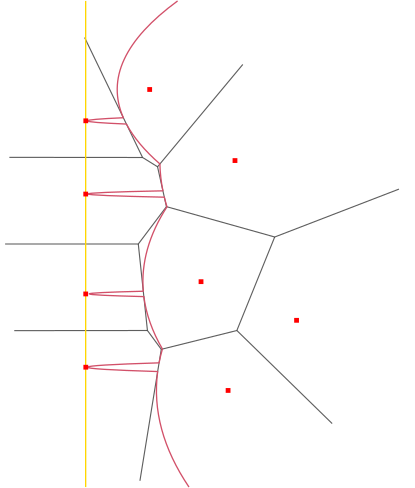
\includegraphics[width=0.48\textwidth]{algolunch/example}
\end{center}
\end{frame}

\end{document}
